\documentclass[12pt]{article}

% A package for setting layout and margins for your thesis 
\usepackage[a4paper]{geometry}

\usepackage[english, estonian]{babel}

% When you write in Estonian then you want to use text with right character set
% By default LaTeX does not know what to do with õäöu letters. You have to specify
% a correct input and font encoding. For that you have to Google the Web     
%
% For TexShop under MacOS X. The right lines are 
%\usepackage[applemac]{inputenc}
\usepackage[T1]{fontenc}
%
% For Windows and Linux the right magic lines are   
% \usepackage[latin1]{inputenc}
% \usepackage[latin5]{inputenc}
% \usepackage[T1]{fontenc}


% General packages for math in general, theorems and symbols 
% Read ftp://ftp.ams.org/ams/doc/amsmath/short-math-guide.pdf for further information
\usepackage{amsmath} 
\usepackage{amsthm}
\usepackage{amssymb}

% Packages for building tables and tabulars 
\usepackage{array}
\usepackage{tabu}   % Wide lines in tables
\usepackage{xspace} % Non-eatable spaces in macros

% Including graphical images and setting the figure directory
\usepackage{graphicx}
\graphicspath{{figures/}}

% Packages for getting clickable links in PDF file
\usepackage{hyperref}
\usepackage[all]{hypcap}

% Packages for defining colourful text together with some colours
\usepackage{color}
\usepackage{xcolor} 
%\definecolor{dkgreen}{rgb}{0,0.6,0}
%\definecolor{gray}{rgb}{0.5,0.5,0.5}
\definecolor{mauve}{rgb}{0.58,0,0.82}

% Standard package for drawing algorithms
% Since the thesis in article format we must define \chapter for
% the package algorithm2e (otherwise obscure errors occur) 
\let\chapter\section
\usepackage[ruled, vlined, linesnumbered]{algorithm2e}

% Fix a  set of keywords which you use inside algorithms
\SetKw{True}{true}
\SetKw{False}{false}
\SetKwData{typeInt}{Int}
\SetKwData{typeRat}{Rat}
\SetKwData{Defined}{Defined}
\SetKwFunction{parseStatement}{parseStatement}

% Nice todo notes
\usepackage{todonotes}

% Proper way to create coloured code listings
\usepackage{listings}
\lstset{ 
  %language=python,                % the language of the code
  language=C++,
  basicstyle=\footnotesize,        % the size of the fonts that are used for the code
  %numbers=left,                   % where to put the line-numbers
  %numberstyle=\footnotesize,      % the size of the fonts that are used for the line-numbers
  numberstyle=\tiny\color{gray}, 
  stepnumber=1,                    % the step between two line-numbers. If it's 1, each line 
                                   % will be numbered
  numbersep=5pt,                   % how far the line-numbers are from the code
  backgroundcolor=\color{white},   % choose the background color. You must add \usepackage{color}
  showspaces=false,                % show spaces adding particular underscores
  showstringspaces=false,          % underline spaces within strings
  showtabs=false,                  % show tabs within strings adding particular underscores
  frame = lines,
  %frame=single,                   % adds a frame around the code
  rulecolor=\color{black},		   % if not set, the frame-color may be changed on line-breaks within 
                                   % not-black text (e.g. commens (green here))
  tabsize=2,                       % sets default tabsize to 2 spaces
  captionpos=b,                    % sets the caption-position to bottom
  breaklines=true,                 % sets automatic line breaking
  breakatwhitespace=false,         % sets if automatic breaks should only happen at whitespace
  %title=\lstname,                 % show the filename of files included with \lstinputlisting;
                                   % also try caption instead of title
                                   % also try caption instead of title
  keywordstyle=\color{blue},       % keyword style
  commentstyle=\color{dkgreen},    % comment style
  stringstyle=\color{mauve},       % string literal style
  escapeinside={\%*}{*)},          % if you want to add a comment within your code
  morekeywords={*,game, fun}       % if you want to add more keywords to the set
}


% Obscure packages to write logic formulae and program semantics
% Unless you do a bachelor thesis on program semantics or static code analysis you do not need that
% http://logicmatters.net/resources/ndexamples/proofsty3.html <= writing type rules => use semantic::inference
% ftp://tug.ctan.org/tex-archive/macros/latex/contrib/semantic/semantic.pdf
\usepackage{proof}
\usepackage{semantic} 
\setlength{\inferLineSkip}{4pt}
\def\predicatebegin #1\predicateend{$\Gamma \vdash #1$}

% If you really want to draw figures in LaTeX use packages tikz or pstricks
% However, getting a corresponding illustrations is really painful  

% Define your favorite macros that you use inside the thesis 
% Name followed by non-removable space
\newcommand{\proveit}{ProveIt\xspace}

% Macros that make sure that the math mode is set
\newcommand{\typeF}[1] {\ensuremath{\mathsf{type_{#1}}}\xspace}
\newcommand{\opDiv}{\ensuremath{\backslash \mathsf{div}}\xspace} 

% Nice Todo box
\newcommand{\TODO}{\todo[inline]}

% A way to define theorems and lemmata
\newtheorem{theorem}{Theorem}


%%% BEGIN DOCUMENT
\begin{document}

% BEGIN TITLE PAGE
\thispagestyle{empty}
\begin{center}

\large
UNIVERSITY OF TARTU\\[2mm]
Institute of Computer Science\\
Computer Science Curriculum\\[2mm]

%\vspace*{\stretch{5}}
\vspace{25mm}

\Large Sten Sootla

\vspace{4mm}

\huge Analysing information distribution in complex systems

%\vspace*{\stretch{7}}
\vspace{20mm}

\Large Bachelor's Thesis (9 ECTS)

\end{center}

\vspace{2mm}

\begin{flushright}
 {
 \setlength{\extrarowheight}{5pt}
 \begin{tabular}{r l} 
  \sffamily Supervisor: & \sffamily Raul Vicente Zafra, PhD \\
  \sffamily Supervisor: & \sffamily Dirk Oliver Theis, PhD
 \end{tabular}
 }
\end{flushright}

%\vspace*{\stretch{3}}
\vspace{10mm}

%{\noindent Author: .................................................................................... ``.....'' ..........\hskip16pt 2048}
\vspace{2mm}


%{\noindent Supervisor: ............................................................................... ``.....'' ..........\hskip16pt 2048}

\vspace{2mm}

%{\noindent Supervisor: ............................................................................... ``.....'' ..........\hskip16pt 2048}

\vspace{8mm}


\vfill
\centerline{Tartu 2017}

% END TITLE PAGE

\selectlanguage{english}

\newpage
\tableofcontents

\newpage
\section{Introduction}

Complex systems 

In Chapter 1, the basics of classical information theory and partial information decomposition are covered. The chapter ends with an overview of the numerical estimator for PID.

The subsequent 3 chapters each introduce a specific complex system and the results of measuring information distribution in it. 

Chapter 2 - Elementary Cellular Automata 
Chapter 3 - Ising model 
Chapter 4 - Artificial Neural Networks

In the final, concluding chapter, a summary of the contributions of this thesis is given, alongside suggestions for further work. 

\newpage
\section{Background}

\subsection{Classical information theory}

In order to understand partial information decomposition, which is the mathematical framework that is used in this thesis to analyse complex systems, a solid understanding of basic information theory is essential. This subsection fills that gap, giving a brief overview of the fundamental concepts of information theory. Where appropriate, the rather abstract definitions are further elaborated on by providing the reader with intuitive explanations and concrete examples.

\subsubsection{Entropy}

Entropy is the most fundamental quantity of information theory.\\

Let $X$ be a discrete random variable with possible realizations from the set $\{x_1, x_2, ..., x_n\}$ and a probability mass function $p(x_i) = P\{X = x_i\} \ (i = 1, ..., n)$. Shannon \cite{shannon} defines the \textit{entropy} of $X$ as follows: 

\begin{equation}
H(X) = -\sum_{i=1}^{n} p(x_i) \log_2 p(x_i)
\label{eq:entropy}
\end{equation}

If the base of the logarithm is 2, the units the entropy is measured in are called \textit{bits}. Another common base for the logarithm is Euler's number $e \approx 2.718$, in which case the units of measurment are called \textit{nats}. \\

Intuitively, entropy can be thought of as the average amount of uncertainty one has about a random variable. It is indeed the \textit{average} amount of uncertainty, because the uncertainty of a single relatization of $x_i$ of a random variable $X$ can be quantified by $-log_2 p(x_i)$. Viewed from this angle, the definition of entropy can be rewritten as an expectation of the random variable $-log_2 p(X)$: 

$$H(X) = \mathbb{E} \left[ - \log_2 p(X) \right] = \mathbb{E} \left[ \log_2 \frac{1}{p(X)} \right].$$ \\ 

To see why this intuition should correspond to the mathematical definition, it is instructive to look at a concrete example, inspired by \cite{cover-thomas}. Suppose we have a binary random variable $X$, defined as follows: 

$$X = \begin{cases} 1 & \mbox{with probability } p, \\ 0, & \mbox{with probability } 1-p. \end{cases}$$ \\

Essentially, this random variable encodes a coin toss, where the probability of flipping heads is $p$ and the probability of flipping tails is $1-p$. If $p=0.5$, the coin is considered to be unbiased, otherwise it is called biased. \\

Using equation \ref{eq:entropy}, it is straightforward to calculate the entropy of $X$, given some specific value of $p$. Figure \ref{fig:entropy} graphs the value of $H(X)$ against every possible $p \in \left[ 0, 1 \right]$. When $p \in \{0, 1\}$, then the outcome of the coin toss is completely deterministic, and there is no uncertainty in the outcome. Accordingly, the entropy is 0 at these points. Conversely, when the coin is fair, we are completely uncertain about the outcome, unable to favour neither heads or tails. Again, the mathematical definition and intuition agree, as the entropy is indeed at its maximum when the coin is fair.

\begin{figure} [h]
\begin{center}
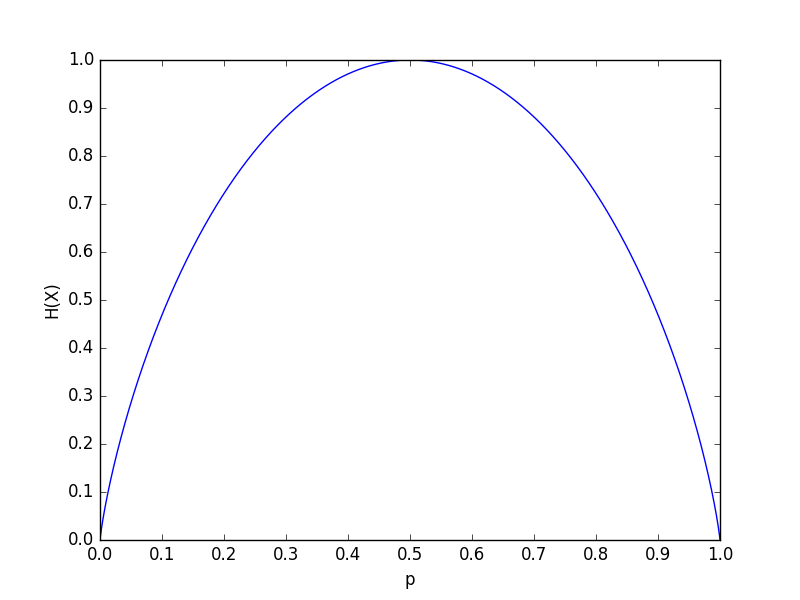
\includegraphics[width=0.8\textwidth]{entropy}
\caption{Entropy of $X$ plotted against the value of $p$.}
\label{fig:entropy}
\end{center}
\end{figure}

The fact that the entropy is maximal when the distribution is uniform is true in general. Another notable property of entropy is that it is non-negative.

\subsubsection{Joint Entropy}

Let $X$ and $Y$ be discrete random variables with realizations from the sets $\{x_1, x_2, ..., x_n\}$ and $\{y_1, y_2, ..., y_n\}$, respectively. Then the \textit{joint entropy} \cite{cover-thomas} of the pair $(X,Y)$ is defined as $$H(X,Y) = -\sum_{i=1}^n \sum_{j=1}^m p(x_i,y_j) log_2 p(x_i,y_j).$$ 

\subsubsection{Conditional entropy}



\subsubsection{Kullback-Leibler distance}

\subsubsection{Mutual information}

Given two discrete random variables $X$ and $Y$, the \textit{mutual information} \cite{cover-thomas} between them is given by $$MI(X;Y) = \sum_{i=1}^n \sum_{j=1}^m p(x,y) \log_2 \frac{p(x,y)}{p(x)p(y)}.$$

\subsubsection{Conditional mutual information}

The \textit{conditional mutual information} \cite{cover-thomas} of discrete random variables $X$ and $Y$ given $Z$ is defined by $$MI(X;Y|Z) = H(X|Z) - H(X|Y,Z) = \mathbb{E}_p(x,y,z) log_2 \frac{p(X,Y|Z)}{p(X|Z)p(Y|Z)}.$$

\subsection{Partial information decomposition}

\subsection{Numerical estimator}

\newpage
\section{Elementary cellular automata}

\subsection{Problem description}
\subsection{Related work}
\subsection{Experimental setup}
\subsection{Results}
\subsection{Discussion}

\newpage
\section{Ising model}

\subsection{Problem description}
\subsection{Related work}
\subsection{Experimental setup}
\subsection{Results}
\subsection{Discussion}

\newpage
\section{Neural networks}

\subsection{Problem description}
\subsection{Related work}
\subsection{Experimental setup}
\subsection{Results}
\subsection{Discussion}

\newpage
\section{Conclusion}


\selectlanguage{english}



\newpage
\bibliographystyle{alpha}
\bibliography{bachelor-thesis}


\appendix
\pagebreak
\section*{\small Non-exclusive licence to reproduce thesis and make thesis public}


I, Sten Sootla (date of birth: 17th of January 1995),

\begin{tabbing}
\= Xiii\=\kill
\>1. \> herewith grant the University of Tartu a free permit (non-exclusive licence) to:\\\\ 

\>1.1\> 
\begin{minipage}[t]{14.2cm}
reproduce, for the purpose of preservation and making available to the public, including for addition to the DSpace digital archives until expiry of the term of validity of the copyright, and
\end{minipage}
\\\\
\>1.2 
\begin{minipage}[t]{14.2cm}
make available to the public via the web environment of the University of Tartu, including via the DSpace digital archives until expiry of the term of validity of the copyright,\\ 

Analysing information distribution in complex systems\\   

supervised by Raul Vicente Zafra and Dirk Oliver Theis

\end{minipage}\\\\ 
\>2. \>I am aware of the fact that the author retains these rights.\\\\
\>3. \>
\begin{minipage}[t]{14.2cm}
I certify that granting the non-exclusive licence does not infringe the intellectual property rights or rights arising from the Personal Data Protection Act. 
\end{minipage}\\
\end{tabbing}

\noindent
Tartu, dd.mm.yyyy


\end{document}

